
\section{Using YAMS - GUI Version}

\subsection{Command Line Options}
To use the GUI version of YAMS, navigate to the directory where the executable is held, and type  YAMS -gui, along with the following options:

\begin{verbatim}
YAMS -gui [-if <file>] | [FILENAMES]
\end{verbatim}

\begin{verbatim}
-if <file>
\end{verbatim}
Input a list of files - the proceeding filename	is a text file containing a list of files that should be executed by the simulator.

\begin{verbatim}
[Filenames]
\end{verbatim}
Input files - One or more input files can be specified to be run by YAMS.  If more than one is specified, they will be run in turn and the output for each displayed in the console window.



The graphical interface will then launch and show the screen below:

\begin{figure}[h]
\centering
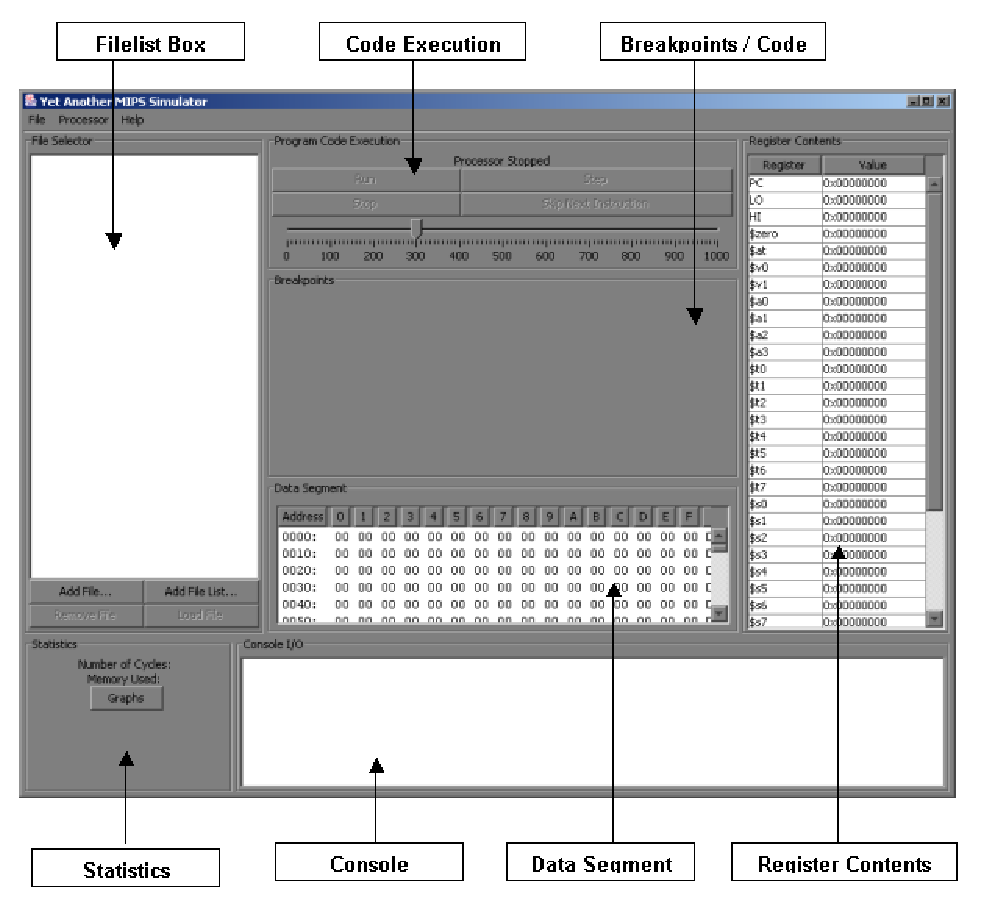
\includegraphics[scale=0.5]{Ch4-Fig2.eps}
\caption{Graphical User Interface}
\label{figure.GUI}
\end{figure}



\subsection{Adding Files to the File Selector Box}
If input files were specified at the command line, they will be displayed in the File Selector Box. Otherwise, files can be added to the File Selector Box by clicking Add File and then using the dialogue box to add a file.

\begin{figure}[h]
\centering
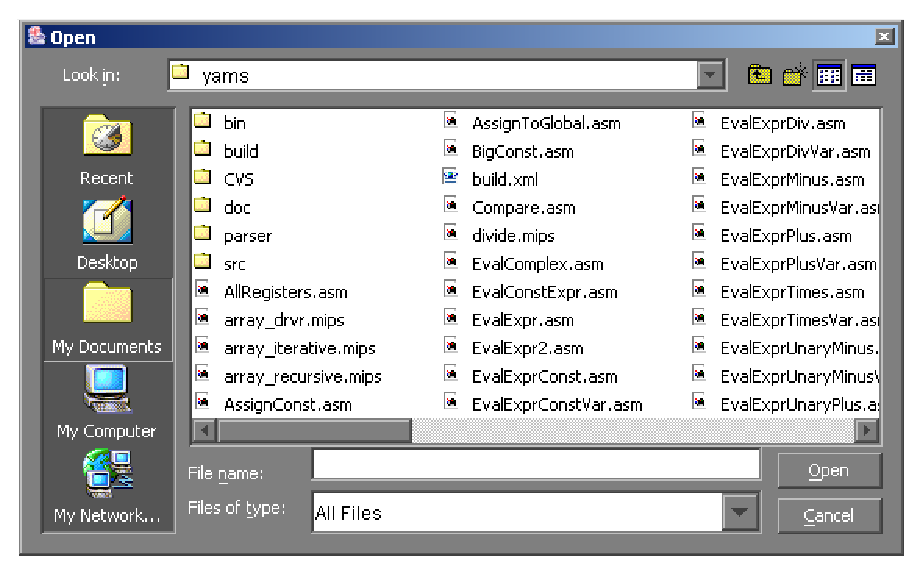
\includegraphics[scale=0.5]{Ch4-Fig3.eps}
\caption{Adding a File}
\label{figure.Adding a File}
\end{figure}

Here you can select an assembly file to load into the simulator.

To add a list of files, click the 'Add Filelist' button, and select the file that contains the list of assembly files you wish to load.  The filelist should contain the file names of the assembly files, one per line.

If you wish to remove a file from the list, select it in the list box, then click the Remove File button below.


\subsection{Loading a File}
Once you have chosen the file you wish YAMS to simulate, you can then load the file by pressing the 'Load File' button.

The program code, memory locations and register contents are shown once the file is loaded, as can be seen below, with the first line of code highlighted.

\begin{figure}[h]
\centering
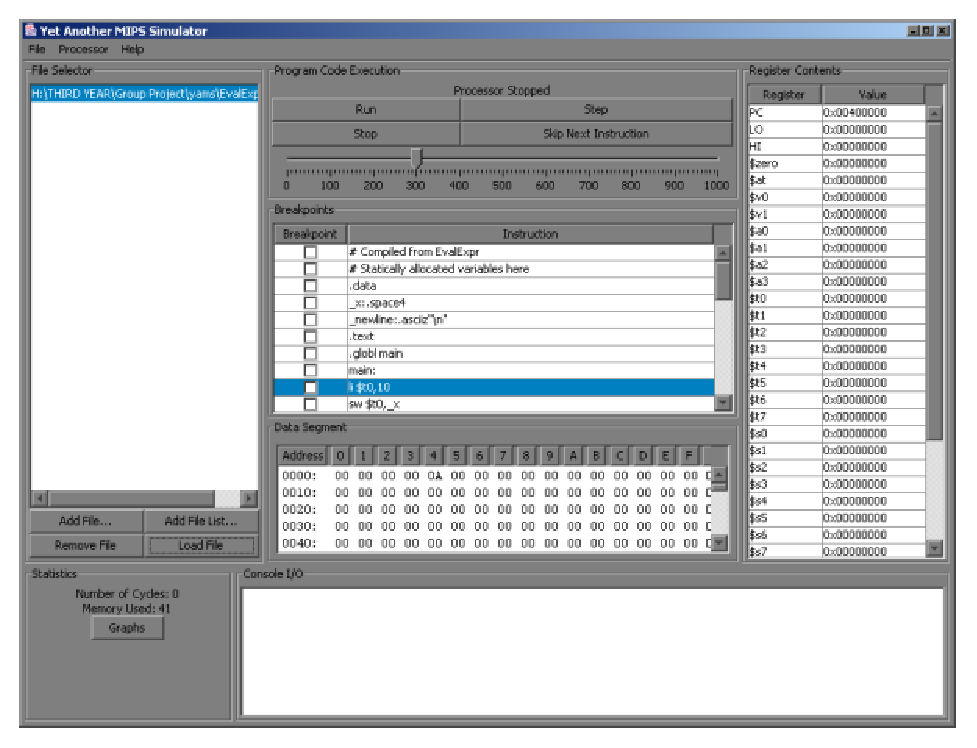
\includegraphics[scale=0.5]{Ch4-Fig4.eps}
\caption{Loading a File}
\label{figure.Loading a File}
\end{figure}


\subsection{Adding Breakpoints}
Adding a breakpoint to the program is simple.  Just use the checkbox that is next to the line you where you wish to pause execution.  When the simulator reaches here, you can examine  the contents of the register and memory locations.

\subsection{Controlling Execution}

\begin{figure}[h]
\centering
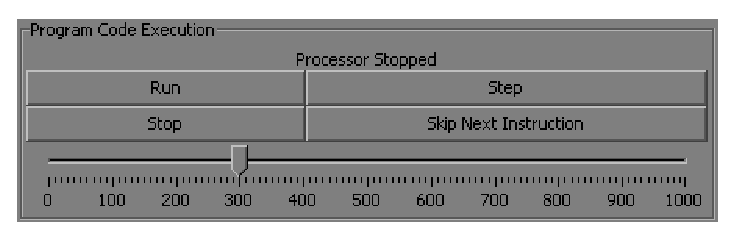
\includegraphics[scale=0.5]{Ch4-Fig5.eps}
\caption{Controlling Execution}
\label{figure.Controlling Execution}
\end{figure}

\subsubsection{Speed}
The speed of the processor can be controlled by the slider bar - a larger value means a longer gap between each instruction so you are able to execute the program in 'slow motion'.  

\subsubsection{Run}
Press the Run button to begin the execution of the assembly program.  The execution of the program is done slowly line by line so that you can see each line being executed individually and the contents of the registers and memory changing.  The current line being executed is shown by the highlighted line in the program code.

\subsubsection{Stop}
To Stop the execution of the program, press the 'Stop' button.  The instruction that is currently being executed will remain highlighted.  From here, it is possible to resume the execution of the program by pressing 'Run', run just the next instruction by pressing 'Step' or skip the next instruction by pressing the 'Skip Next Instruction' button.

\subsubsection{Single Step}
If you wish to single step each line of the program, first of all, press the Stop button which will pause the programs execution.  It is then possible to use the Step button to execute each instruction one at a time.  Note that one line of assembly code can be made up of several processor operations, so pressing Step will not always move to the next instruction, but will execute the next processor operation for that line.

\subsubsection{Skip}
Pressing 'Skip Next Instruction' will ignore the next insturction that is to be executed.  It is recommended that this feature is used while in stepping mode so that it can be seen clearly which instruction is to be skipped.


\subsection{Interpreting Output}


\subsubsection{Console Output}
The Console I/O box is used for 2 things:
- Error messages from the parser - if an error was encountered while parsing the assmebly file, the type of error and related line number are displayed.  Correct the error then try loading the file again.

- Output of the program - during the execution of the program, any output is displayed in the Console I/O box.

\subsubsection{Statistics}
Statistics for the run of the program are available in the Statistics Panel of the interface.  This shows the number of CPU cycles required so far for the program executing, and the total amount of memory used by the program.  These are updated constantly as the program is executed.

\begin{figure}[h]
\centering
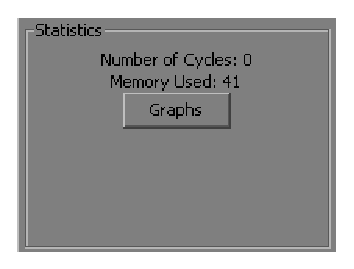
\includegraphics[scale=0.5]{Ch4-Fig6.eps}
\caption{Statistics Panel}
\label{figure.Statistics Panel}
\end{figure}


Pressing the 'Graph' button will display a window with 2 tabs:
- How many times each register was used
- How many times each line was executed

This can be useful in seeing where loops are in the program as the lines in the loop are executed more often than the rest of the instructions.

